\documentclass[UTF8,zihao=-4]{ctexart}

\usepackage[a4paper,top=2.6cm,bottom=2.4cm,left=2.6cm,right=2.6cm]{geometry}
\usepackage{graphicx}
\usepackage{booktabs}
\usepackage{array}
\usepackage{longtable}
\usepackage{float}
\usepackage{caption}
\usepackage{subcaption}
\usepackage{amsmath}
\usepackage{amssymb}
\usepackage{xcolor}
\usepackage{listings}
\usepackage{hyperref}
\usepackage{enumitem}
\usepackage{fancyhdr}
\usepackage{setspace}
\usepackage{tabularx}

\hypersetup{
  colorlinks=true,
  linkcolor=black,
  citecolor=black,
  urlcolor=blue
}

\graphicspath{{figures/}}
\setstretch{1.22}
\setlength{\parindent}{2em}
\setlength{\parskip}{0.25em}
\setlength{\headheight}{15pt}
\emergencystretch=3em
\captionsetup{font=small,labelfont=bf}
\pagestyle{fancy}
\fancyhf{}
\fancyhead[L]{机器学习实验报告}
\fancyhead[R]{基于 kNN 的手写数字识别}
\fancyfoot[C]{\thepage}

\definecolor{codebg}{RGB}{247,247,247}
\definecolor{codegray}{RGB}{80,80,80}
\lstdefinestyle{pythonstyle}{
  language=Python,
  basicstyle=\ttfamily\small,
  keywordstyle=\color{blue!70!black},
  commentstyle=\color{codegray},
  stringstyle=\color{green!40!black},
  numbers=left,
  numberstyle=\tiny\color{codegray},
  stepnumber=1,
  numbersep=8pt,
  backgroundcolor=\color{codebg},
  showstringspaces=false,
  breaklines=true,
  frame=single,
  rulecolor=\color{black!20},
  tabsize=4
}

\newcommand{\course}{机器学习}
\newcommand{\reporttitle}{实验一：基于 kNN 的手写数字识别}
\newcommand{\studentname}{尚文轩}
\newcommand{\studentid}{2412456}
\newcommand{\major}{计算机科学与技术}

\begin{document}

\begin{titlepage}
  \centering
  \vspace*{2.8cm}
  {\fontsize{30}{40}\selectfont\bfseries \course\ 实验报告\par}
  \vspace{1.2cm}
  {\fontsize{24}{34}\selectfont\bfseries \reporttitle\par}
  \vspace{2.8cm}
  {\fontsize{16}{24}\selectfont
  \renewcommand{\arraystretch}{1.6}
  \begin{tabular}{>{\bfseries}r l}
    姓名： & \studentname \\
    学号： & \studentid \\
    专业： & \major \\
    实验数据集： & Semeion 手写数字数据集 \\
    完成日期： & 2026 年 10 月 9 日
  \end{tabular}\par}
  \vspace{1.2cm}
  {\fontsize{13}{20}\selectfont\bfseries GitHub 仓库\par}
  \vspace{0.3cm}
  {\fontsize{12}{18}\selectfont
  \url{https://github.com/ZR-1N/Machine_Learning_NKU}\par}
  \vfill
  {\large 南开大学\par}
\end{titlepage}

\clearpage
\pagenumbering{Roman}
\tableofcontents
\clearpage
\pagenumbering{arabic}

\section{实验概述}

\subsection{实验目的}

本实验围绕 Semeion 手写数字数据集实现 k 近邻分类器，并使用留一法交叉验证评估模型效果。结合课程导论文档与 kNN 课件，本实验的目标包括：

\begin{enumerate}[label=\arabic*.]
  \item 理解 kNN 作为监督学习算法的基本思想，掌握距离度量、近邻数量 $k$、投票规则等关键因素对分类结果的影响。
  \item 使用 Python 与 NumPy 自行实现欧氏距离、多数表决和留一法交叉验证，不依赖现成分类器完成核心实验。
  \item 使用 Weka 的 IBk 分类器复现实验，并比较自写程序与 Weka 的分类精度。
  \item 分析实验中出现的数据格式、评估协议、默认参数和平局处理等问题，形成可复现、可解释的实验结论。
\end{enumerate}

\subsection{实验内容与进阶要求}

基础任务要求实现自写 kNN 和 LOO 评估，并对 $k=1,3,5$ 进行实验。中级要求使用 Weka 进行对照实验。进阶要求不仅记录运行结果，还需要说明思考过程、具体实现步骤和踩坑记录。因此，本报告在常规的算法原理、实现方法、实验结果之外，专门加入数据准备验证、Weka 参数对齐、预期值异常排查和误差来源分析。

\section{数据集与实验环境}

\subsection{数据集说明}

实验使用 Semeion Handwritten Digit 数据集。原始文件为 \texttt{semeion.data}，共 1593 行、266 列。每行前 256 列表示 $16 \times 16$ 二值手写数字图像展开后的像素，后 10 列表示 one-hot 编码标签。设原始行向量为
\[
  \mathbf{r} = (x_1,\ldots,x_{256}, y_0,\ldots,y_9),
\]
其中 $x_i \in \{0,1\}$，标签由
\[
  c = \arg\max_{j \in \{0,\ldots,9\}} y_j
\]
得到。

本地检查结果显示，数据矩阵形状为 $(1593,266)$，类别分布如表 \ref{tab:class-dist} 所示。各类别样本数量接近，适合用于比较不同 $k$ 值下的整体分类效果。

\begin{table}[H]
  \centering
  \caption{Semeion 数据集类别分布}
  \label{tab:class-dist}
  \begin{tabular}{ccccccccccc}
    \toprule
    类别 & 0 & 1 & 2 & 3 & 4 & 5 & 6 & 7 & 8 & 9 \\
    \midrule
    样本数 & 161 & 162 & 159 & 159 & 161 & 159 & 161 & 158 & 155 & 158 \\
    \bottomrule
  \end{tabular}
\end{table}

\subsection{数据文件关系验证}

实验文件夹中同时存在完整数据 \path{semeion.data} 以及两份划分文件 \path{semeion_train.txt}、\path{semeion_test.txt}。起初容易误以为训练集和测试集划分文件也应参与本实验。实际核对后可知，训练文件有 1293 行，测试文件有 300 行，二者合计 1593 行；用 NumPy 将二者拼接后按行排序，与 \path{semeion.data} 的行集合完全一致。因此，train/test 文件只是全集的一个划分版本。

由于导论文档第 5 节要求使用留一法，LOO 的定义是每次从完整数据集中留出一个样本测试，其余样本训练，所以本实验只使用 \texttt{semeion.data}。这一点直接影响实验协议：如果改用固定 train/test 划分，样本数量、评估方式和结果都不能与 LOO 对齐。

\subsection{实验环境}

\begin{table}[H]
  \centering
  \caption{实验环境与工具}
  \label{tab:env}
  \begin{tabularx}{\textwidth}{>{\bfseries}l X}
    \toprule
    项目 & 配置或用途 \\
    \midrule
    操作系统 & Windows 环境下运行 Python 与 Weka \\
    Python 依赖 & NumPy 用于矩阵运算，Matplotlib 用于图像展示 \\
    核心程序 & \texttt{exp\_1.py} 实现 kNN 与 LOO，\texttt{knn.py} 展示样本图像 \\
    Weka 工具 & Weka Explorer 中的 \texttt{lazy.IBk} 分类器 \\
    数据转换 & \texttt{convert\_to\_arff.py} 将空格分隔数据转换为 Weka 原生 ARFF 格式 \\
    \bottomrule
  \end{tabularx}
\end{table}

原始运行截图显示程序在名为 \texttt{ml} 的 Python 环境中执行，但没有记录 Python 与 NumPy 的具体版本。报告修订阶段的复核环境为 Python 3.12.7、NumPy 1.26.4；该环境的结果单独列于后文，不与原始记录混用。Weka 版本未在现有截图及文本输出中标明。

\textbf{数据准备的思考与步骤。} 首先明确评估协议，再选择输入文件，以避免将固定训练/测试划分误用于 LOO。具体步骤为：
\begin{enumerate}[label=\arabic*.]
  \item 将完整数据保存在 \path{data/semeion.data}，使用 \texttt{np.loadtxt} 读取，并检查矩阵形状为 $(1593,266)$。
  \item 检查前 256 列的像素取值为 0 或 1，后 10 列为合法独热编码；每行标签区域应恰有一个 1。
  \item 分离特征与标签，得到 $X\in\mathbb{R}^{1593\times256}$ 和 $y\in\{0,\ldots,9\}^{1593}$，统计类别数量。
  \item 比较 train/test 拼接数据与全集的行多重集合，保留重复行的计数；确认一致后，仅将完整数据用于 LOO。
\end{enumerate}

\section{kNN 算法原理}

\subsection{基本思想}

kNN 是一种直观的监督学习方法，可用于分类和回归。它没有显式的参数训练过程，而是在预测阶段计算待分类样本与训练集中所有样本的距离，选出距离最近的 $k$ 个样本，再根据这些近邻的标签进行预测。课件中用“物以类聚，人以群分”概括了这一思想：如果一个样本在特征空间中接近某一类样本，它大概率也属于该类。

对于分类任务，kNN 的三个核心步骤为：

\begin{enumerate}[label=\arabic*.]
  \item 数据准备：读入带标签数据，并将 one-hot 标签转换为整数类别。
  \item 寻找近邻：计算测试样本与所有训练样本的距离，按距离升序排列。
  \item 投票预测：选取前 $k$ 个近邻，以多数表决得到预测类别。
\end{enumerate}

\subsection{距离度量}

本实验使用欧氏距离。设样本 $\mathbf{x}_i,\mathbf{x}_j \in \mathbb{R}^{256}$，则二者距离为
\[
  d(\mathbf{x}_i,\mathbf{x}_j)
  =
  \sqrt{\sum_{m=1}^{256}(x_{im}-x_{jm})^2}.
\]

Semeion 的像素为 0/1 二值特征，因此欧氏距离与汉明距离存在单调关系：平方欧氏距离实际上等于两个二值向量不同位置的数量。使用欧氏距离可以保持与导论代码、Weka 默认距离设置一致。

课件强调不同量纲的特征应归一化。本实验的全部像素具有相同取值范围 $\{0,1\}$，不存在量纲较大的特征支配距离的问题，因此自写程序直接使用原始二值像素。标签只用于投票及评价，不参与距离计算。

\subsection{k 值选择}

$k$ 是 kNN 的关键超参数。$k$ 过小时，模型容易受噪声或异常样本影响，分类边界更不稳定；$k$ 过大时，模型会过度平滑局部结构，可能忽略细粒度差异。课件建议常用 $k=3,5,7$，本实验按照导论文档要求比较 $k=1,3,5$。

\section{自写 kNN 与 LOO 实现}

\subsection{数据读取与标签转换}

核心读取代码如下。前 256 列作为特征矩阵 $X$，后 10 列通过 \texttt{argmax} 转换为 $0$ 到 $9$ 的整数标签。

\begin{lstlisting}[style=pythonstyle,caption={数据读取与标签转换}]
raw = np.loadtxt('data/semeion.data')
X = raw[:, :256]
y = np.argmax(raw[:, 256:], axis=1)
\end{lstlisting}

\subsection{向量化距离计算}

LOO 需要进行 1593 轮评估。每一轮中，一个样本作为测试样本，其余 1592 个样本作为训练样本。若使用纯 Python 双重循环，需要大约
\[
  1593 \times 1592 \times 256 \approx 6.5 \times 10^8
\]
次逐维计算，运行时间会明显增加。因此，实验中使用 NumPy 广播一次性计算测试样本到所有训练样本的距离：

\begin{lstlisting}[style=pythonstyle,caption={欧氏距离的向量化实现}]
def euclidean_distances(X_train, x_test):
    squares = (X_train - x_test) ** 2
    dists = np.sqrt(squares.sum(axis=1))
    return dists
\end{lstlisting}

这里 \texttt{X\_train - x\_test} 会自动将一维测试向量按行广播到训练矩阵上，从而得到所有训练样本与测试样本的逐维差值。该实现简洁且高效，是本实验完成 LOO 的关键。

\subsection{多数表决与平局规则}

预测阶段先对距离排序，取前 $k$ 个近邻标签，再使用 \texttt{np.bincount().argmax()} 得到票数最多的类别：

\begin{lstlisting}[style=pythonstyle,caption={kNN 预测函数}]
def knn_predict(X_train, y_train, x_test, k):
    dists = euclidean_distances(X_train, x_test)
    k_idx = np.argsort(dists)[:k]
    k_labels = y_train[k_idx]
    pred = np.bincount(k_labels).argmax()
    return pred
\end{lstlisting}

需要注意的是，\texttt{argmax()} 在多个类别票数相同时返回编号最小的类别。这是一个确定性的平局规则，但不一定与 Weka 完全相同。对于二值像素数据，距离并列很常见，平局规则会在 $k=3$ 等情况下造成小幅结果差异。

导论允许在投票平局时随机选取类别，本实现采用编号最小者，便于固定投票结果。奇数 $k$ 并不能保证多分类任务没有平局，例如 $k=3$ 时三个邻居分别属于不同类别，仍会出现 $1$--$1$--$1$ 的票数并列。此外，\texttt{np.argsort} 默认排序不保证等距离样本的相对顺序，因此投票规则固定并不等于近邻集合跨环境完全固定。

\subsection{留一法交叉验证}

LOO 的实现如下。每轮删除第 $i$ 个样本作为测试样本，其余样本用于预测，最后统计正确率。

\begin{lstlisting}[style=pythonstyle,caption={LOO 评估函数}]
def loo_eval(X, y, k):
    n = X.shape[0]
    correct = 0
    for i in range(n):
        x_test = X[i]
        X_train = np.delete(X, i, axis=0)
        y_train = np.delete(y, i)
        pred = knn_predict(X_train, y_train, x_test, k)
        if pred == y[i]:
            correct += 1
    return correct / n
\end{lstlisting}

\textbf{评估指标与数据隔离。} 设第 $i$ 轮预测为 $\hat y_i$，则
\[
  \mathrm{Acc}_{\mathrm{LOO}}=\frac{1}{1593}\sum_{i=1}^{1593}\mathbf{1}(\hat y_i=y_i).
\]
每个样本恰好被测试一次，且在对应轮次中不属于训练集。若不删除测试样本，样本自身会以零距离参与近邻搜索，导致评估失真。LOO 衡量逐样本留出的识别效果；数据没有在本实验中按书写者划分，因此结果不能直接解释为对全新书写者的识别性能。

\textbf{实现思路与执行步骤。} 采用三个函数分别负责距离计算、投票预测和评估，以便检查错误来自哪个环节。
\begin{enumerate}[label=\arabic*.]
  \item 编写距离函数，用广播完成逐维相减，沿特征轴求和，返回长度为 1592 的距离向量。
  \item 编写预测函数，对距离排序，选取前 $k$ 个下标，统计对应标签并输出多数类别。
  \item 编写 LOO 函数，按同一下标同时删除特征行和标签，防止训练数据与标签错位。
  \item 对 $k=1,3,5$ 分别遍历全集，统计预测正确次数，以总样本数为分母计算准确率。
  \item 在项目根目录运行 \texttt{python exp\_1.py}，保存控制台输出并截图，核对样本数量与三个 $k$ 值。
\end{enumerate}

主流程与结果输出如下：
\begin{lstlisting}[style=pythonstyle,caption={不同 k 值的评估主流程}]
if __name__ == '__main__':
    for k in [1, 3, 5]:
        acc = loo_eval(X, y, k)
        print(f'k={k}  LOO accuracy = {acc:.4f}')
\end{lstlisting}
上例仅将输出文字写为英文，评估调用与源码一致。距离计算总量为 $O(n^2d)$，逐轮完整排序还需要 $O(n^2\log n)$ 的工作量，其中 $n=1593$、$d=256$。向量化减少 Python 层面的循环开销，并未改变距离计算的渐近复杂度。当前实现每轮还通过 \texttt{np.delete} 复制训练数据；规模进一步扩大时，可考虑距离缓存或批量计算，并明确距离并列的处理规则。

\section{样本可视化与数据检查}

\subsection{导论示例代码运行情况}

导论文档给出的样本展示代码注释写的是“随机画 6 张图”，但原代码使用 \texttt{for i in range(6)} 取固定前 6 行。实际文件中前 20 个样本的标签均为 0，因此每次展示的前 6 张图都标为 0。数字 0 的总样本数为 161，这不表示前 161 行全部属于数字 0。图 \ref{fig:sample-display} 展示了固定取样现象。

\begin{figure}[H]
  \centering
  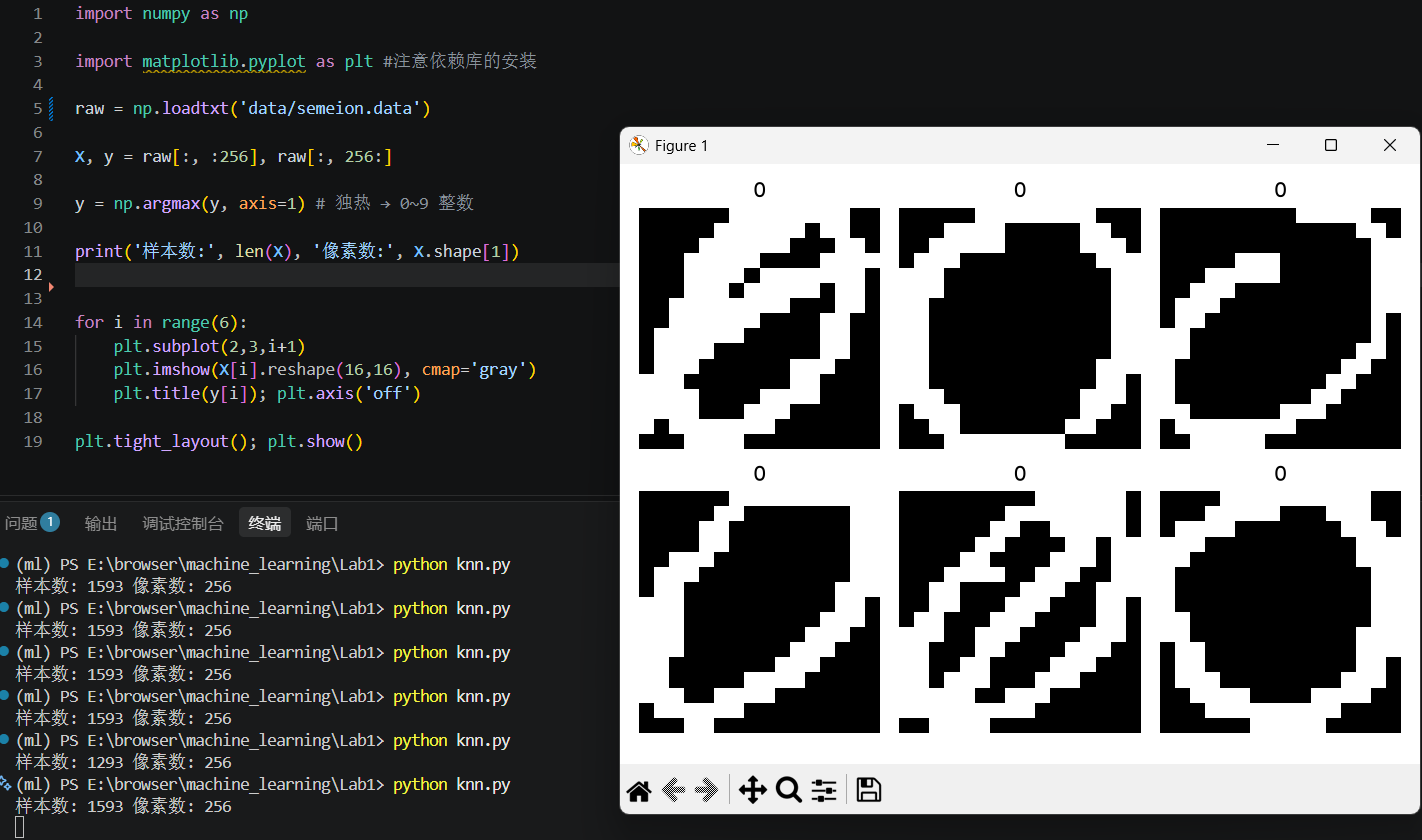
\includegraphics[width=0.92\textwidth]{sample_display.png}
  \caption{导论示例代码运行结果：固定展示前 6 个样本}
  \label{fig:sample-display}
\end{figure}

逐行检查表明，前 6 个像素向量彼此不同，属于六个不同样本；现有数据没有提供可供本实验核查的书写者标识，不能据此断定来自六位不同书写者。若希望真正随机展示样本，可采用以下修正写法。本报告截图仍为原始示例的固定取样结果。

\begin{lstlisting}[style=pythonstyle,caption={随机抽样展示 6 张图像的修正写法}]
idx = np.random.choice(len(X), 6, replace=False)
for pos, i in enumerate(idx):
    plt.subplot(2, 3, pos + 1)
    plt.imshow(X[i].reshape(16, 16), cmap='gray')
    plt.title(y[i])
    plt.axis('off')
\end{lstlisting}

\textbf{可视化的思考与步骤。} 展示图像用于检查像素排列和标签解码，而不能替代对全部数据的合法性检查。执行时先运行 \texttt{python knn.py}，确认控制台显示 1593 个样本、256 个像素；再将选中的 256 维向量恢复为 $16\times16$，使用统一灰度色图并以真实标签作为标题，保存截图。随机展示时可固定随机种子以便复现，但该抽样只改变展示内容，不改变 LOO 输入数据及评估结果。

\section{Weka 对比实验}

\subsection{ARFF 转换}

Weka 不能直接将 \texttt{semeion.names} 当作数据文件读取。\texttt{.names} 文件只是数据集说明，Weka 会按 C4.5 的属性定义文件解析，因而报出格式错误。同时，原始 \texttt{semeion.data} 是空格分隔文本，也不是 Weka 最稳定的输入格式。为保证 Weka 正确识别属性和类别，本实验使用脚本转换为 ARFF：

\begin{lstlisting}[style=pythonstyle,caption={ARFF 转换的关键结构}]
lines.append('@relation semeion_handwritten_digit')
for i in range(256):
    lines.append(f'@attribute p{i+1} numeric')
lines.append('@attribute class {0,1,2,3,4,5,6,7,8,9}')
lines.append('@data')
for row, label in zip(X, y):
    pixels = ','.join(str(int(v)) for v in row)
    lines.append(pixels + f',{int(label)}')
with open('data/semeion.arff', 'w', encoding='utf-8') as f:
    f.write('\n'.join(lines))
\end{lstlisting}

其中 256 个像素属性声明为 \texttt{numeric}，类别属性声明为 nominal 类型 \texttt{\{0,1,2,3,4,5,6,7,8,9\}}。若类别也被当成 numeric，Weka 可能无法按分类任务正确处理。

\subsection{Weka 参数设置}

Weka Explorer 中选择 \texttt{lazy.IBk}。为了与自写代码可比，设置如下：

\begin{itemize}
  \item \texttt{KNN} 分别设为 1、3、5。
  \item \texttt{DistanceFunction} 使用 \texttt{EuclideanDistance}。
  \item \texttt{distanceWeighting} 设置为 \texttt{No distance weighting}；记录的命令行没有启用 \texttt{-I} 或 \texttt{-F} 加权选项。
  \item \texttt{windowSize} 为 0，即不限制训练池大小，对应 \texttt{-W 0}。该参数与距离加权无关。
  \item 不启用 IBk 内部自动选择 $k$ 的 \texttt{crossValidate} 选项，以保持每次运行指定的 $k$ 值。
  \item \texttt{Cross-validation folds} 设置为 1593，使每折只留出一个样本，等价于 LOO。
\end{itemize}

根据 Weka 的 IBk 官方参数说明，\texttt{-I} 表示按距离倒数加权，\texttt{-F} 表示按 $1-d$ 加权，\texttt{-W} 表示训练池窗口大小。实验应核对实际配置，不将距离倒数加权视为必然的默认设置。若启用加权投票，就与自写程序的等权投票不同。IBk 内部选择 $k$ 的交叉验证和 Explorer 的外部性能评估也属于不同设置。

\textbf{对比实验的思考与操作步骤。} 对比的前提是使用相同样本、特征、类别定义及外部评估协议，而不仅是设置相同 $k$。
\begin{enumerate}[label=\arabic*.]
  \item 在项目根目录运行 \texttt{python convert\_to\_arff.py}，生成 \path{data/semeion.arff}。
  \item 打开 Weka Explorer，在 Preprocess 页通过 Open file 导入 ARFF，检查 Instances 为 1593、Attributes 为 257，并将最后一列 nominal 属性 \texttt{class} 设为目标类别。
  \item 在 Classify 页选择 \texttt{lazy.IBk}，将 KNN 设为 1，检查距离函数、投票方式及窗口设置。
  \item 在 Test options 中选择 Cross-validation，将 Folds 设为 1593，然后 Start；检查输出 Test mode 为 1593-fold cross-validation。
  \item 记录正确/错误分类数、准确率和混淆矩阵，将输出保存为文本并截图；分别设置 KNN 为 3、5 后重复运行。
  \item 对照每次输出内部的 \texttt{Scheme} 或所选结果记录识别对应的 $k$，再填写比较表。截图顶部显示的是当前待运行配置，未必是当前选中的历史结果配置。
\end{enumerate}

\section{实验结果}

\subsection{自写程序结果}

原始本地运行截图如图 \ref{fig:local-loo} 所示，与 \path{loo.txt} 中的记录一致。表 \ref{tab:local-result} 据此整理，保留输出的四位小数。

\begin{figure}[H]
  \centering
  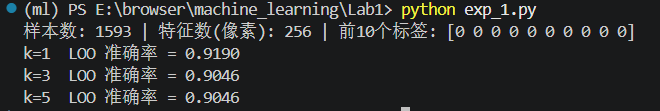
\includegraphics[width=0.98\textwidth]{local_loo.png}
  \caption{自写程序的原始本地 LOO 运行结果}
  \label{fig:local-loo}
\end{figure}

\begin{table}[H]
  \centering
  \caption{自写 kNN 在 LOO 下的准确率}
  \label{tab:local-result}
  \begin{tabular}{ccc}
    \toprule
    $k$ & LOO 准确率 & 正确率百分比 \\
    \midrule
    1 & 0.9190 & 91.90\% \\
    3 & 0.9046 & 90.46\% \\
    5 & 0.9046 & 90.46\% \\
    \bottomrule
  \end{tabular}
\end{table}

结果显示，$k=1$ 在本实现中表现最好。随着 $k$ 从 1 增至 3 或 5，准确率下降约 1.44 个百分点，说明在该数据集和欧氏距离设置下，较小的局部邻域更能保留手写数字图像的细节差异。

\subsection{Weka 结果}

Weka 对 $k=1,3,5$ 的结果分别如图 \ref{fig:weka-k1}、图 \ref{fig:weka-k3}、图 \ref{fig:weka-k5} 所示。

\begin{figure}[H]
  \centering
  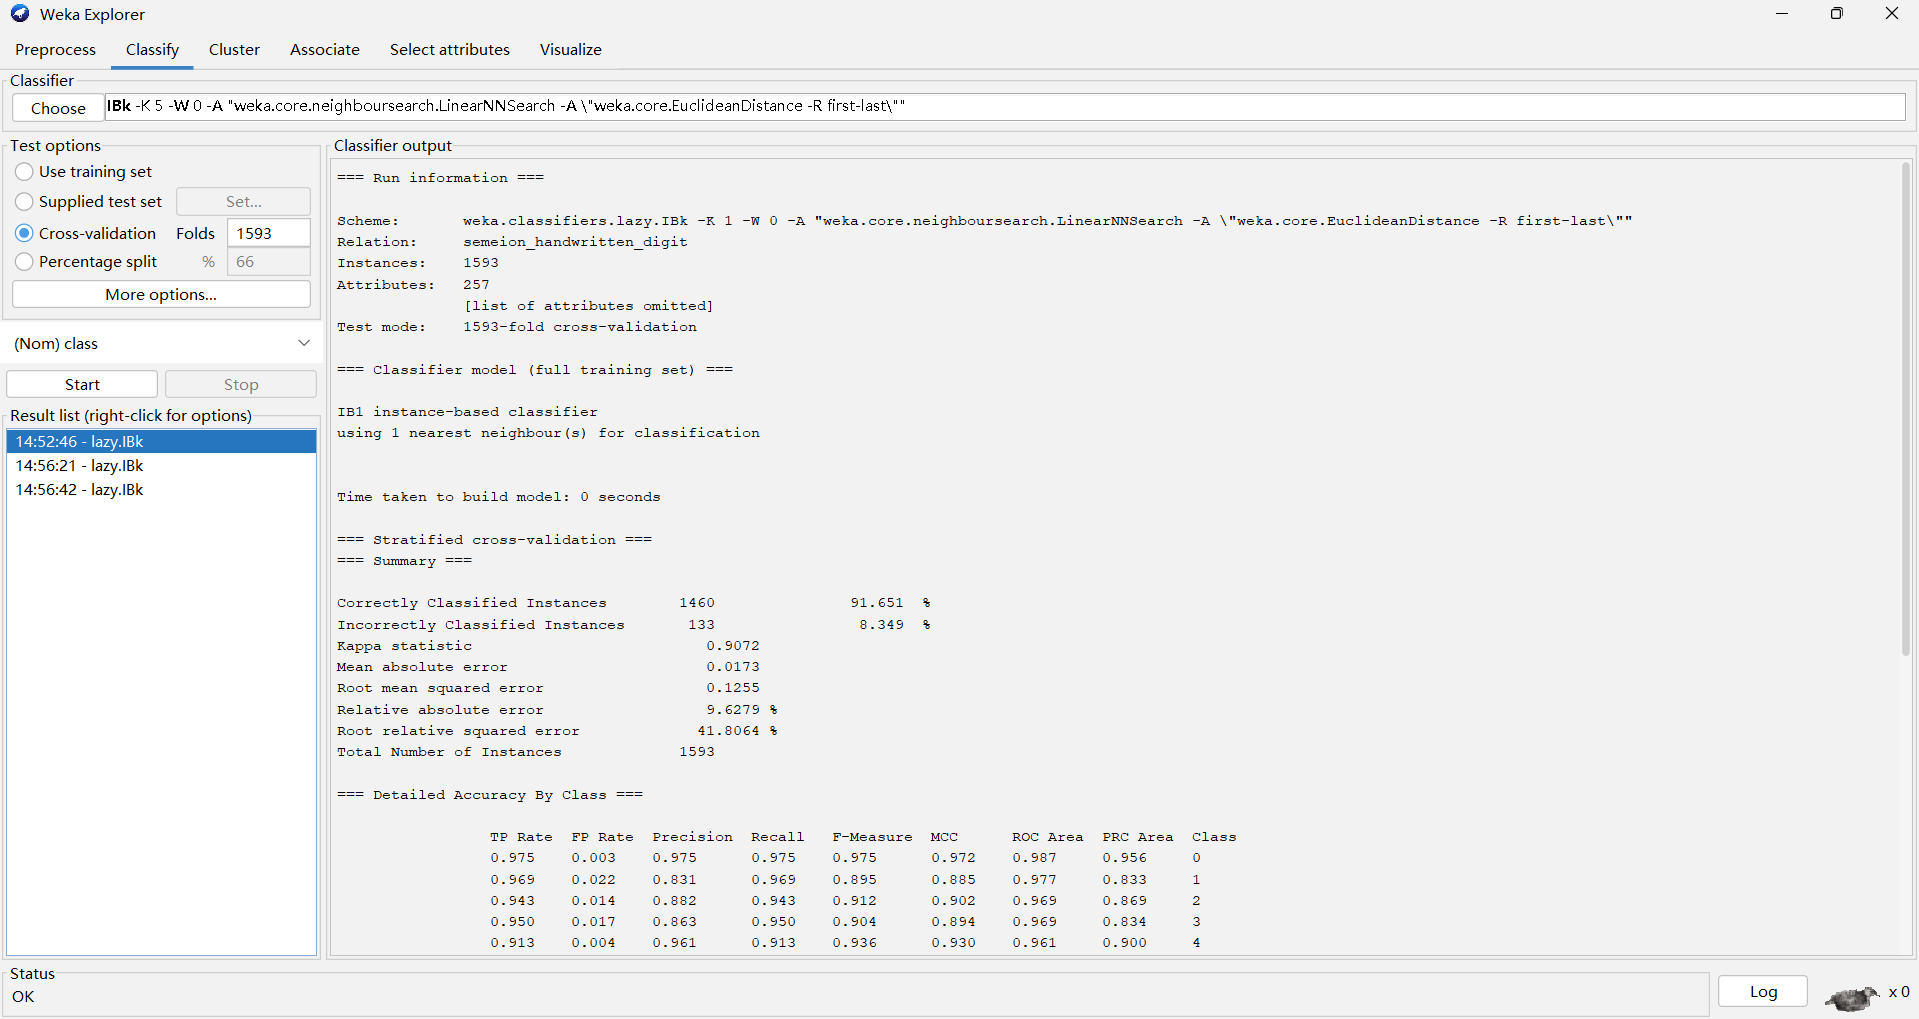
\includegraphics[width=0.98\textwidth]{weka_k1.png}
  \caption{Weka IBk 在 $k=1$ 时的 LOO 结果}
  \label{fig:weka-k1}
\end{figure}

\begin{figure}[H]
  \centering
  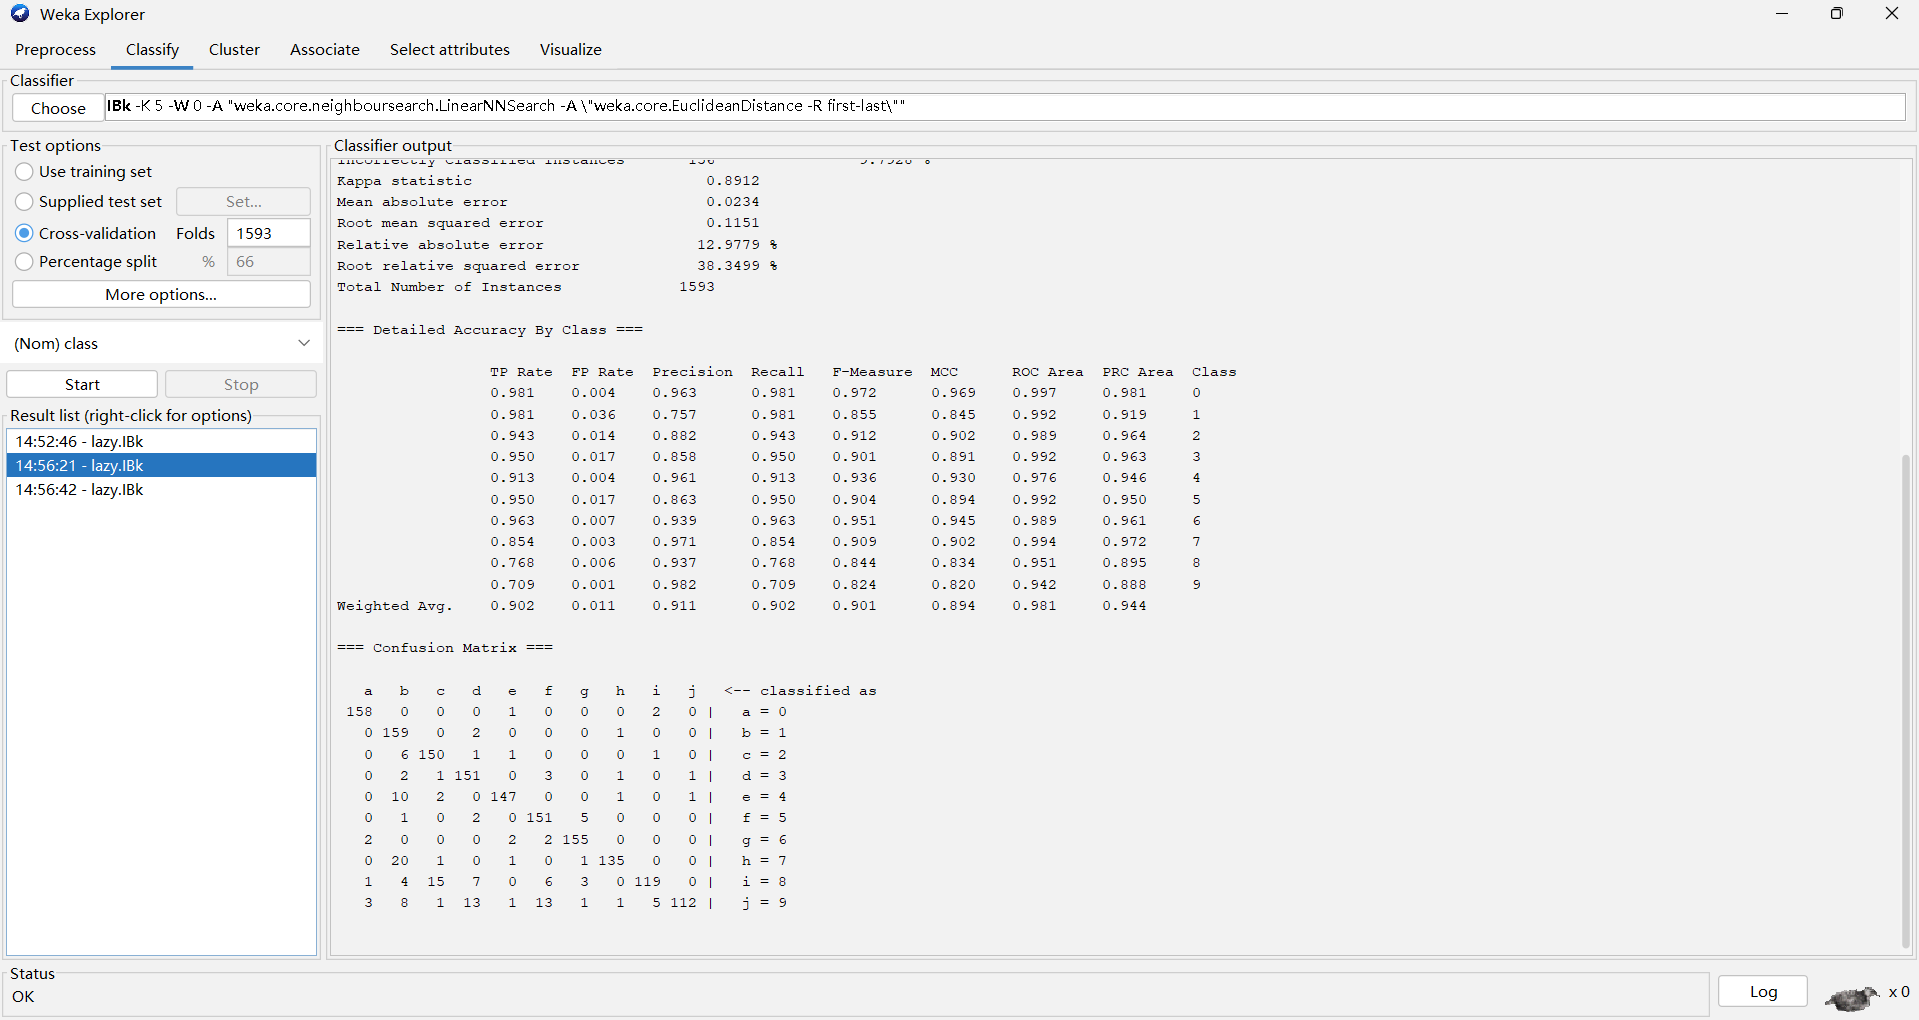
\includegraphics[width=0.98\textwidth]{weka_k3.png}
  \caption{Weka IBk 在 $k=3$ 时的 LOO 结果}
  \label{fig:weka-k3}
\end{figure}

\begin{figure}[H]
  \centering
  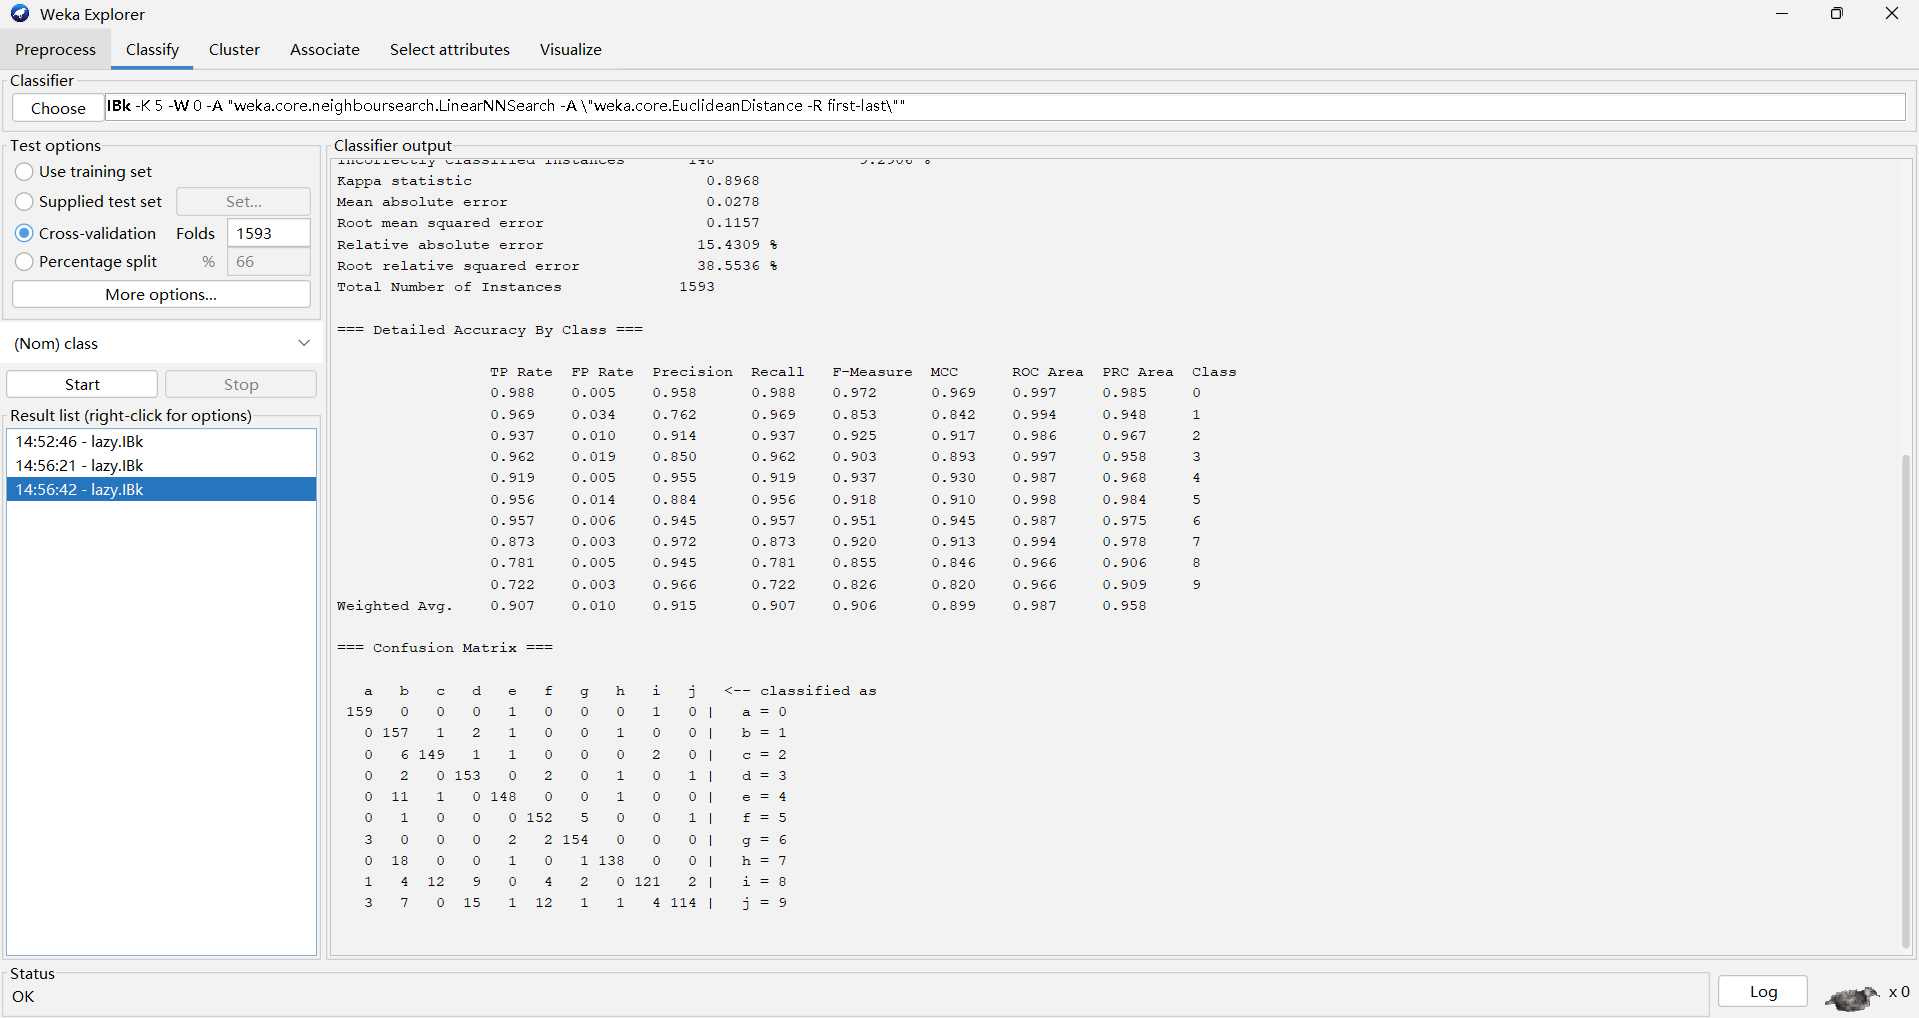
\includegraphics[width=0.98\textwidth]{weka_k5.png}
  \caption{Weka IBk 在 $k=5$ 时的 LOO 结果}
  \label{fig:weka-k5}
\end{figure}

Weka 文本输出中的核心指标如表 \ref{tab:weka-result} 所示。

\begin{table}[H]
  \centering
  \caption{Weka IBk 的 LOO 准确率}
  \label{tab:weka-result}
  \begin{tabular}{cccc}
    \toprule
    $k$ & 正确分类数 & 错误分类数 & 准确率 \\
    \midrule
    1 & 1460 & 133 & 91.6510\% \\
    3 & 1437 & 156 & 90.2072\% \\
    5 & 1445 & 148 & 90.7094\% \\
    \bottomrule
  \end{tabular}
\end{table}

\subsection{自写程序与 Weka 对比}

\begin{table}[H]
  \centering
  \caption{自写 kNN 与 Weka IBk 结果对比}
  \label{tab:compare}
  \begin{tabular}{cccc}
    \toprule
    $k$ & 自写 LOO 精度 & Weka LOO 精度 & 差异（百分点） \\
    \midrule
    1 & 91.90\% & 91.6510\% & 0.2490 \\
    3 & 90.46\% & 90.2072\% & 0.2528 \\
    5 & 90.46\% & 90.7094\% & 0.2494 \\
    \bottomrule
  \end{tabular}
\end{table}

按显示精度计算，三组结果的绝对差异均小于 0.5 个百分点，未触发导论中“差异超过阈值时说明原因”的条件。差异仍可能与两类实现细节有关：一是二值像素存在等距离样本，近邻集合在边界处可能不同；二是投票平局规则可能不同。准确率接近支持整体结果的一致性，但没有 Weka 的逐样本预测和近邻记录，不能将这些可能解释认定为已经确定的原因。

\section{实验结果验证与分析}

\subsection{文档预期值与实际结果不一致}

导论文档给出的预期输出约为 98.5\%，而本实验在 LOO、欧氏距离和多数表决设置下得到约 91\% 的准确率。为分析差异来源，从实现逻辑、数据完整性、工具配置和评估协议四个方面进行核查。

排查过程如下：

\begin{enumerate}[label=\arabic*.]
  \item 验证代码：检查欧氏距离、标签索引、测试样本排除及准确率分母。实验者另报告曾使用 scikit-learn 进行独立验证，$k=1$ 约为 0.917；该验证的源码、版本和完整输出未包含在现有材料中，因此作为辅助说明，不作为本报告表格的数值依据。
  \item 验证数据：本地计算 \path{semeion.data} 的 MD5 为 \texttt{cb545d371d2ce14ec121\allowbreak470795a77432}，并确认 train/test 合并后与全集一致。
  \item 验证工具：Weka 使用 ARFF 输入、欧氏距离、无距离加权、1593 折交叉验证，得到与自写程序小于 0.5\% 的差异。
  \item 验证协议：依据文本输出核对 Weka 为 1593 折评估，依据源码确认自写程序每轮留出一行。现有材料没有包含其他距离和评估方式的完整实验记录，因此不将“所有变体均无法达到预期值”作为已验证结论。
\end{enumerate}

上述核查表明，自写程序与 Weka 的结果一致性较高，导论文档中的预期值未能在当前数据及实验协议下复现。现有证据尚不足以确定该预期值的来源，因此本报告以本地运行记录和 Weka 输出为依据，报告实测结果。

\subsection{补充复核与排序敏感性}

在 Python 3.12.7、NumPy 1.26.4 环境下直接执行现有 \texttt{exp\_1.py}，得到 0.9159、0.9065、0.9052，与原始截图有所不同。为进一步检查近邻排序的影响，保持数据、欧氏距离、LOO 与投票规则不变，仅将 \texttt{np.argsort(dists)} 替换为 \texttt{np.argsort(dists, kind='stable')} 进行补充复核，结果如表 \ref{tab:sort-audit}。该复核不修改提交源码，也不替代原始实验记录。

\begin{table}[H]
  \centering
  \caption{修订阶段不同距离排序规则的复核结果}
  \label{tab:sort-audit}
  \begin{tabular}{ccccc}
    \toprule
    $k$ & 默认排序正确数 & 准确率 & 稳定排序正确数 & 准确率 \\
    \midrule
    1 & 1459 & 91.5882\% & 1461 & 91.7137\% \\
    3 & 1444 & 90.6466\% & 1440 & 90.3955\% \\
    5 & 1442 & 90.5210\% & 1440 & 90.3955\% \\
    \bottomrule
  \end{tabular}
\end{table}

在当前默认排序中，第 $k$ 与第 $k+1$ 个邻居等距的测试样本数分别为 134、342、430；多数投票出现多个最高票类别的样本数分别为 0、45、45。排序切换确实改变了正确分类数，证明近邻边界的距离并列会影响当前数据的结果。NumPy 官方文档指出，默认排序不保证等值元素的相对顺序；稳定排序则保留其原始顺序。稳定排序使近邻选择规则更明确，但仍依赖输入行顺序，不保证获得更高精度。

本次复核与原始记录之间的差异不能仅凭上述检查完全归因，因为原始运行环境的依赖版本及当时源码快照未完整保存。后续复现实验应同时记录 Python/NumPy 版本、数据校验值、源码版本、距离并列与投票平局规则。原始实验与当前复核均得到约 90\%--92\% 的准确率，但应明确区分两个运行批次。

补充复核脚本保存在 \path{report/reproduce_checks.py}。在项目根目录用 Python 执行该脚本后，将生成 \path{report/reproduction_checks.json}，记录环境版本、数据校验值、正确数及两种平局计数。统计逻辑保持原始默认排序预测不变，分别检查近邻边界和最高票类别是否并列。关键代码如下：
\begin{lstlisting}[style=pythonstyle,caption={等距离边界与投票平局的检查方法}]
order = np.argsort(dists)
boundary_tie = dists[order[k - 1]] == dists[order[k]]
counts = np.bincount(y_train[order[:k]], minlength=10)
vote_tie = np.count_nonzero(counts == counts.max()) > 1
stable_order = np.argsort(dists, kind='stable')
stable_pred = np.bincount(y_train[stable_order[:k]]).argmax()
\end{lstlisting}

\subsection{按类别表现分析}

以 Weka 的 $k=1$ 结果为例，数字 0、1、2、3、4、5、6、7 的召回率均超过 0.91，其中数字 0 的精确率与召回率均为 0.975。数字 8 和 9 的召回率相对较低，分别为 0.806 和 0.791。结合混淆矩阵，数字 8 容易被分到 2、3、6、9 等类别，数字 9 容易被分到 3、5 等类别。这与手写数字形状相似性一致：8 的上下环结构在低分辨率二值化后可能与 2 或 6 混淆，9 的闭环和尾部也容易与 3 或 5 混淆。

$k=3$ 与 $k=5$ 时，整体准确率低于 $k=1$，且数字 9 的召回率下降较明显。这说明扩大邻域后，一些局部写法差异被周围不同类别样本“稀释”，尤其影响形状边界较接近的类别。

\clearpage
\subsection{自写分类器的混淆矩阵}

为将总体精度与具体误分类联系起来，在 Python 3.12.7、NumPy 1.26.4 环境下对 $k=1,3,5$ 分别执行完整留一法预测。绘图脚本直接调用 \texttt{exp\_1.py} 的 \texttt{knn\_predict} 函数，并逐轮排除测试样本，保持原程序的距离计算、默认排序和投票规则不变。三个矩阵均来自同一环境下的补充复核运行，与前述复核正确数一致，不对应原始截图或 Weka 的预测记录。错分类样例仍取本批次 $k=1$ 的预测。

设混淆矩阵为 $C$，其中 $C_{ab}$ 表示真实类别为 $a$、预测类别为 $b$ 的样本数。矩阵行对应真实类别，列对应预测类别；对角线为正确分类，非对角线为误分类。图 \ref{fig:local-confusion}、图 \ref{fig:local-confusion-k3} 和图 \ref{fig:local-confusion-k5} 均显示样本计数，色阶统一为 0--160；矩阵元素总和均为 1593，对角线之和依次为 1459、1444、1442。

\begin{figure}[H]
  \centering
  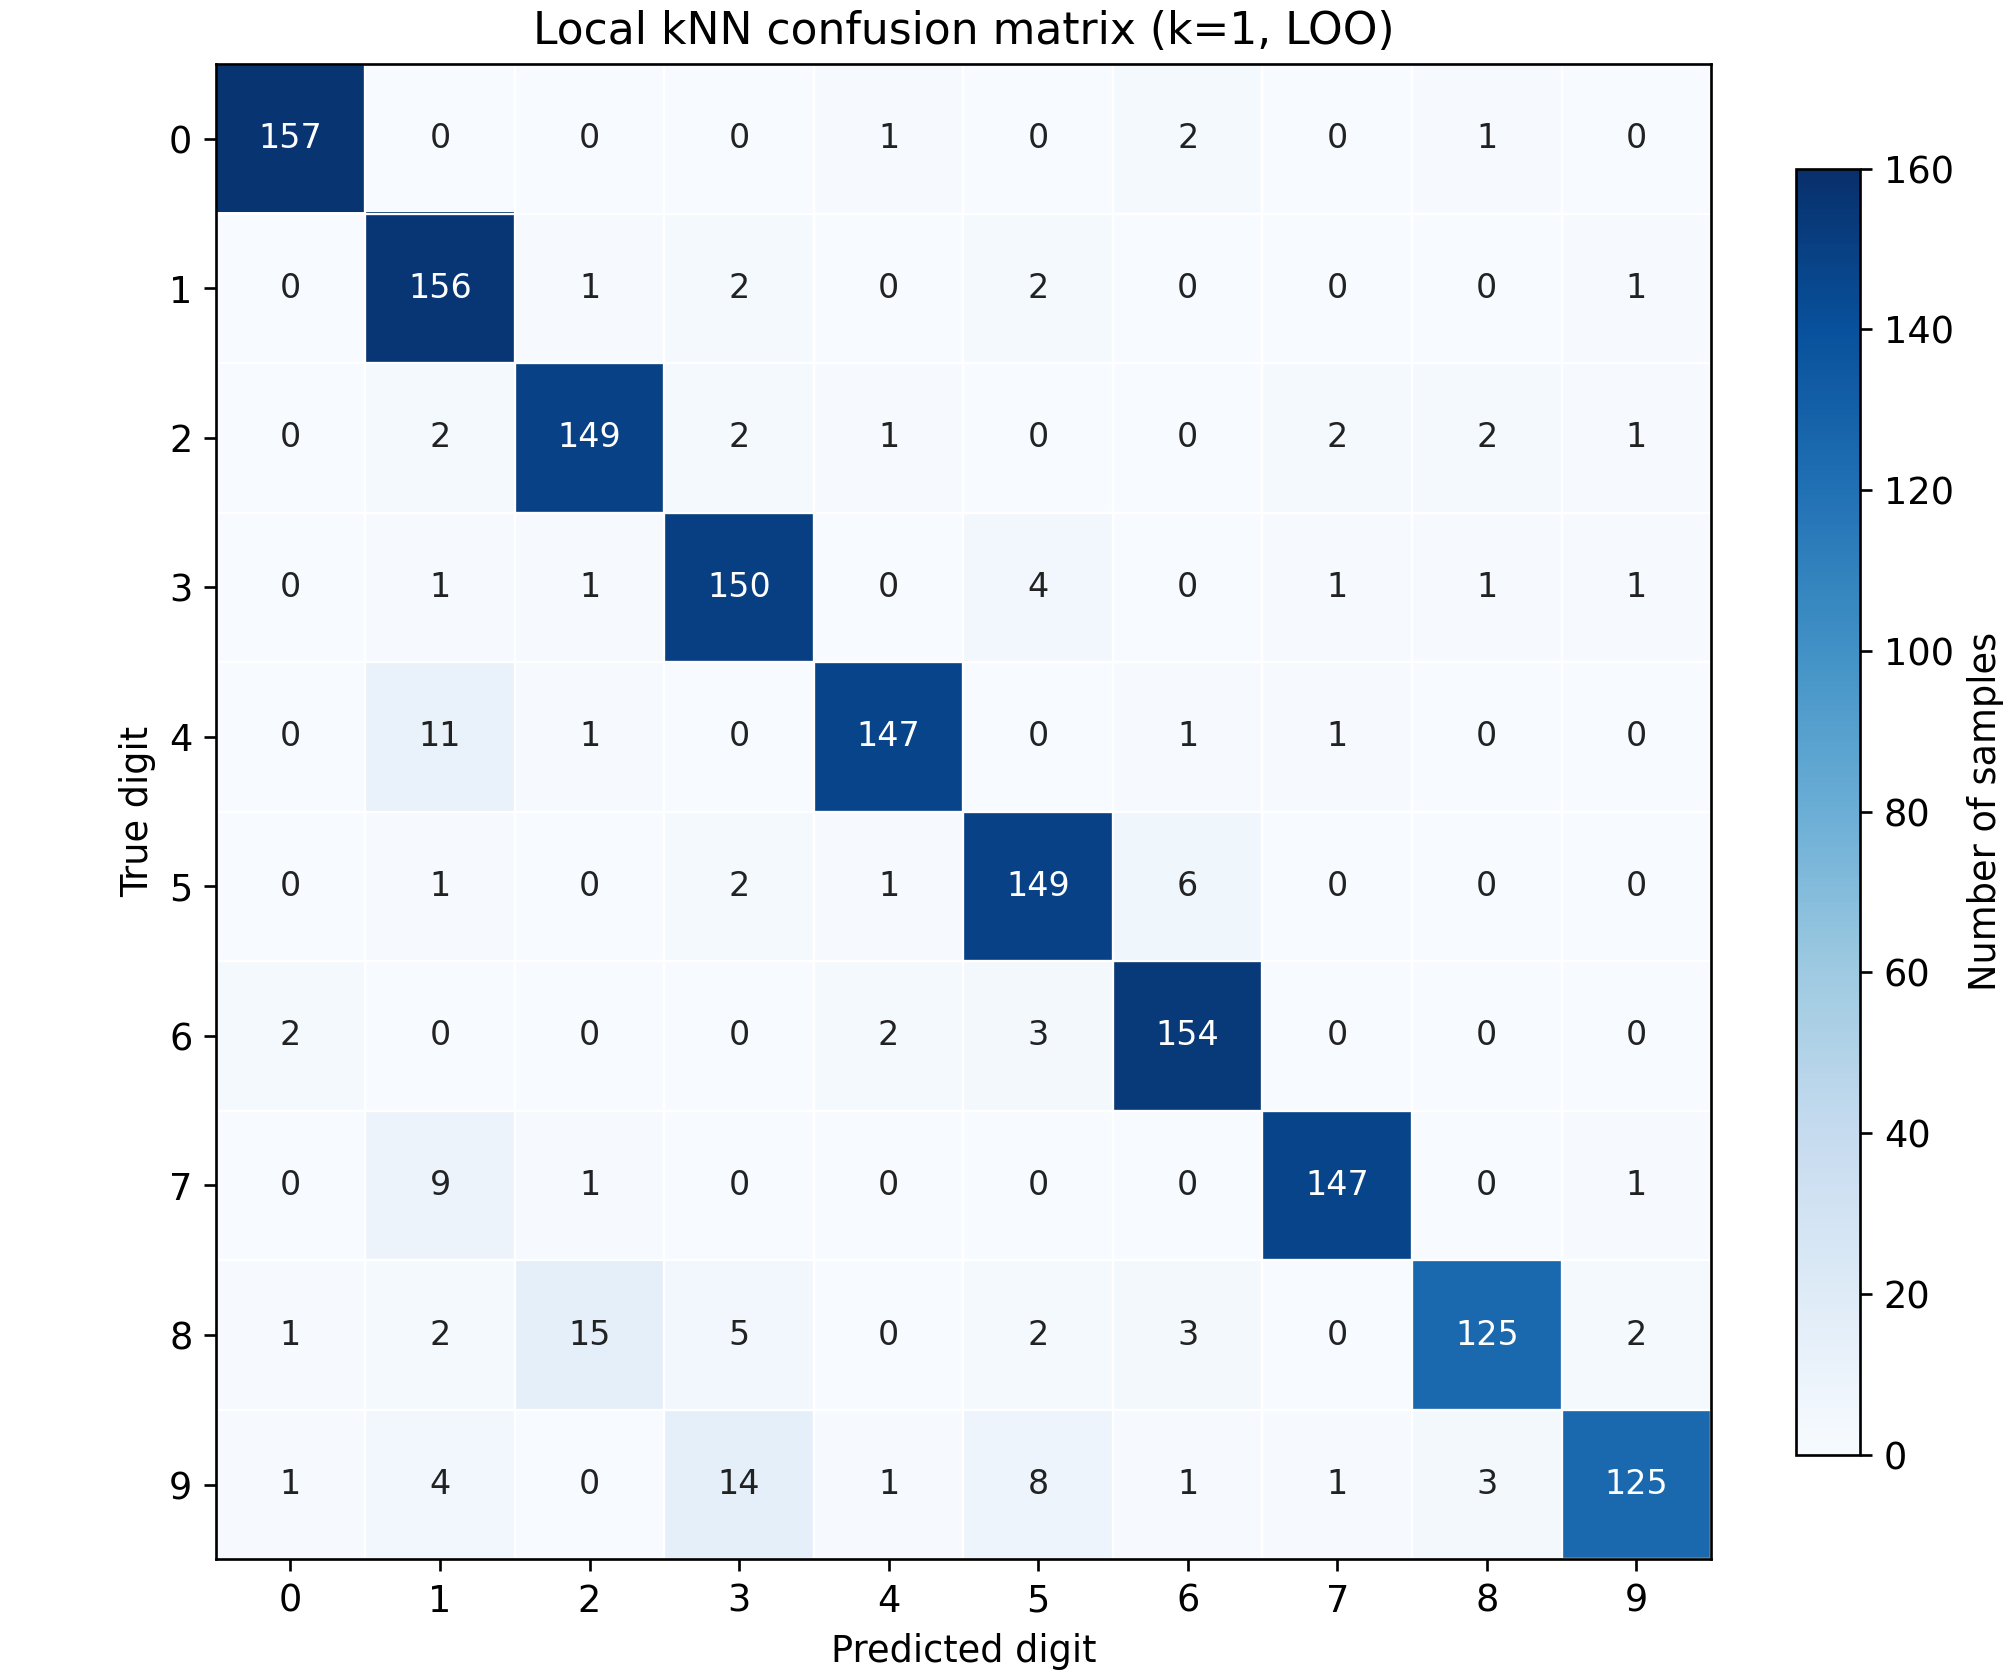
\includegraphics[width=0.83\textwidth]{local_confusion_k1.png}
  \caption{自写 kNN 的 $k=1$ LOO 混淆矩阵：补充复核运行，行是真实类别、列是预测类别}
  \label{fig:local-confusion}
\end{figure}

数字 8 和 9 的召回率分别为 $125/155=80.6452\%$ 和 $125/158=79.1139\%$，低于其他类别。最大非对角项为 $8\rightarrow2$（15 次），其次为 $9\rightarrow3$（14 次）和 $4\rightarrow1$（11 次）。这些计数说明总体错误集中于若干相近类别，也与 Weka 的主要混淆趋势一致；不过两套实现的矩阵不是完全相同的预测记录。

\clearpage
\textbf{$k=3$ 的混淆矩阵。} 本次正确分类 1444 个、错误分类 149 个，准确率为 90.6466\%。图 \ref{fig:local-confusion-k3} 展示各类别的具体去向。

\begin{figure}[H]
  \centering
  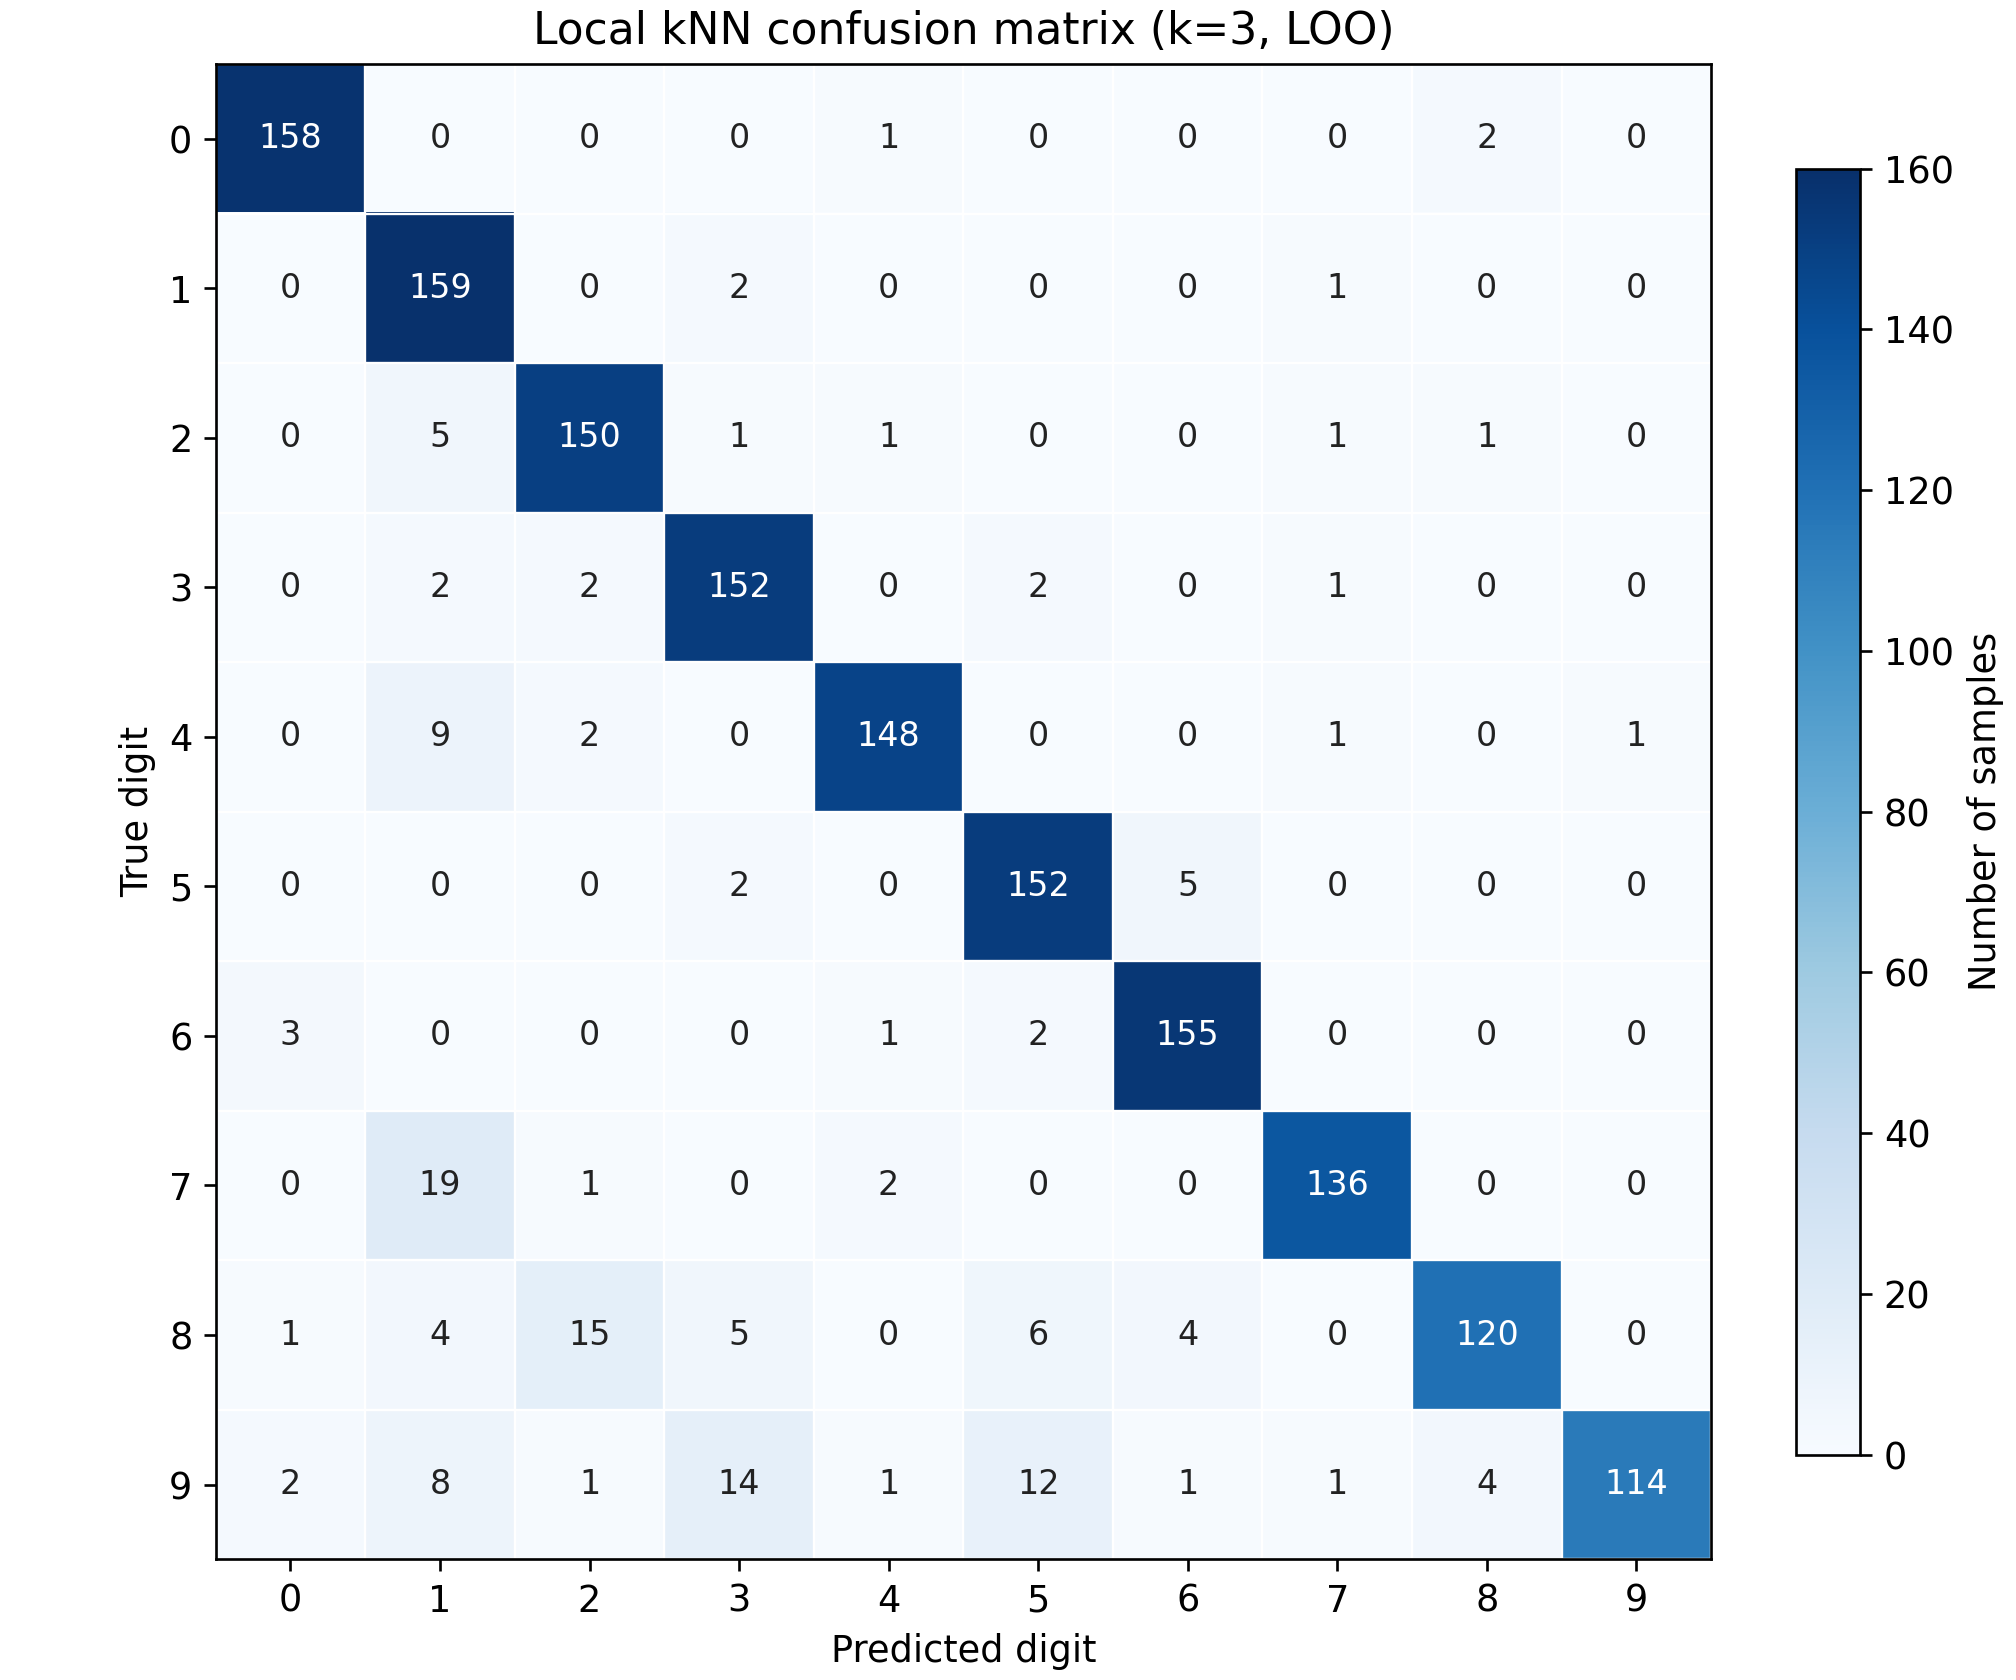
\includegraphics[width=0.90\textwidth]{local_confusion_k3.png}
  \caption{自写 kNN 的 $k=3$ LOO 混淆矩阵：补充复核运行，行是真实类别、列是预测类别}
  \label{fig:local-confusion-k3}
\end{figure}

相较 $k=1$，数字 0、1、2、3、4、5、6 的正确分类数有所增加，但数字 7、8、9 的正确数分别由 147、125、125 降为 136、120、114。其中 $7\rightarrow1$ 的错误由 9 次增至 19 次，$9\rightarrow5$ 由 8 次增至 12 次，$8\rightarrow2$ 仍为 15 次。这表明增加邻居数量带来的改善并不均匀：部分类型受益于投票，而易混淆类型的损失使总体精度下降。

\clearpage
\textbf{$k=5$ 的混淆矩阵。} 本次正确分类 1442 个、错误分类 151 个，准确率为 90.5210\%。图 \ref{fig:local-confusion-k5} 与另外两图使用相同轴定义和色阶。

\begin{figure}[H]
  \centering
  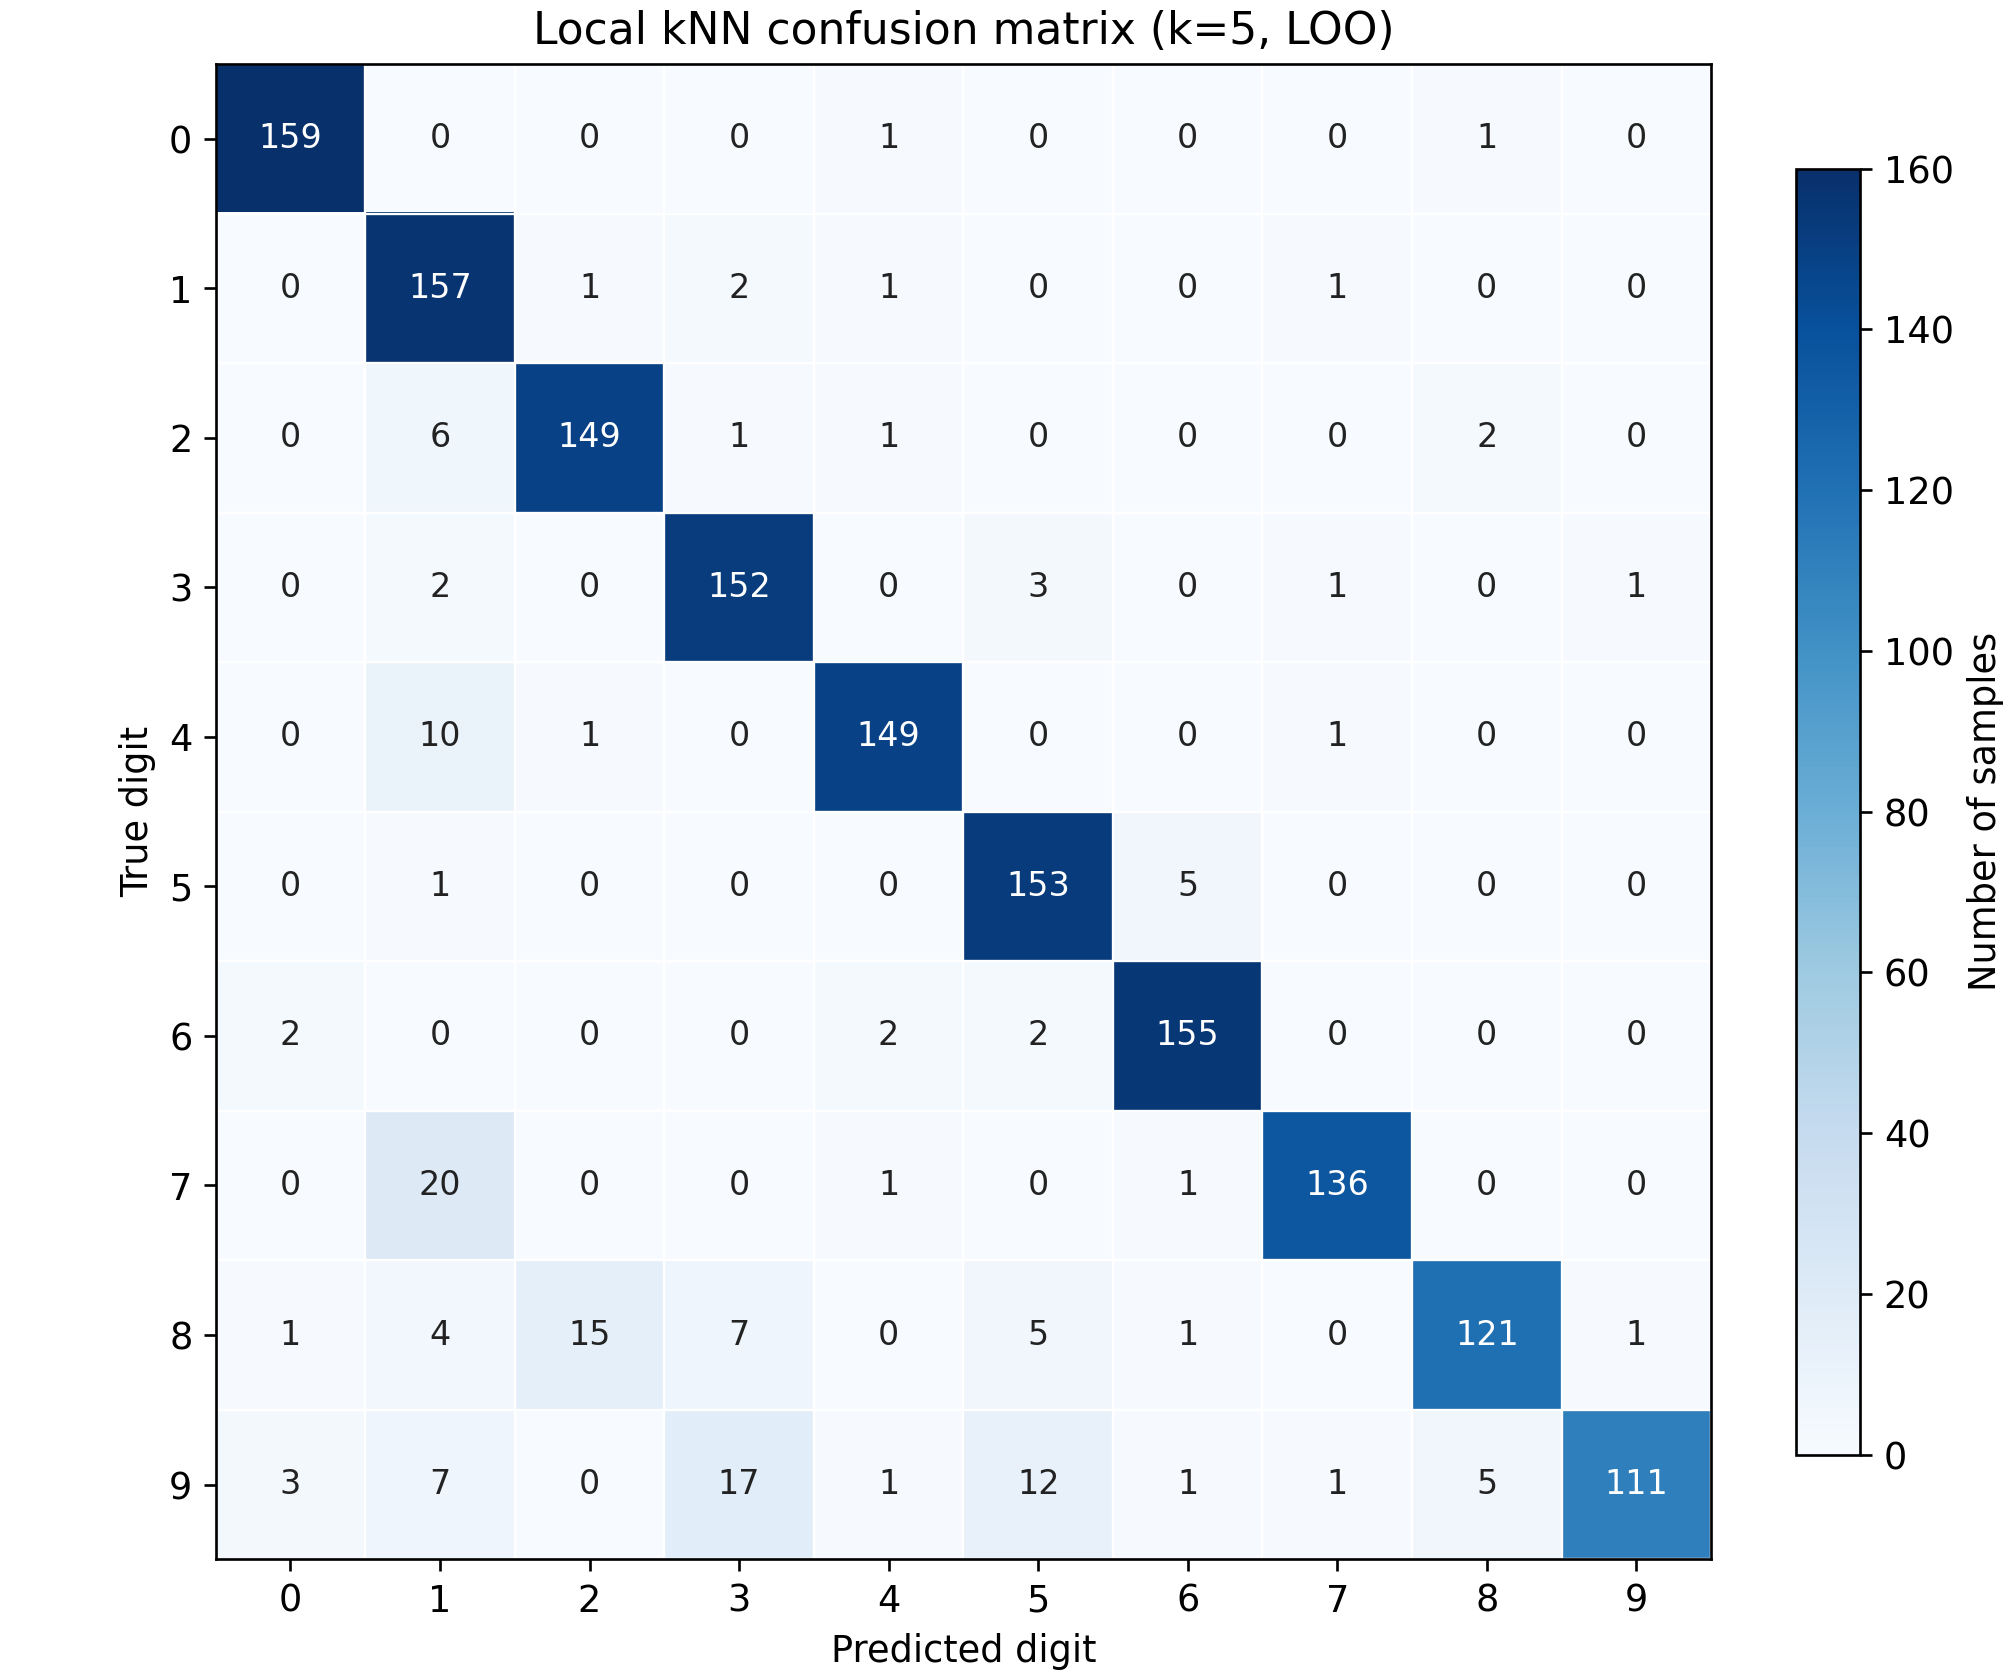
\includegraphics[width=0.88\textwidth]{local_confusion_k5.png}
  \caption{自写 kNN 的 $k=5$ LOO 混淆矩阵：补充复核运行，行是真实类别、列是预测类别}
  \label{fig:local-confusion-k5}
\end{figure}

\begin{table}[H]
  \centering
  \caption{同一补充运行中不同 k 的整体精度及易混淆类别召回率}
  \label{tab:confusion-recall}
  \begin{tabular}{ccccc}
    \toprule
    $k$ & 准确率 & 数字 7 召回率 & 数字 8 召回率 & 数字 9 召回率 \\
    \midrule
    1 & 91.5882\% & 93.0379\% & 80.6452\% & 79.1139\% \\
    3 & 90.6466\% & 86.0759\% & 77.4194\% & 72.1519\% \\
    5 & 90.5210\% & 86.0759\% & 78.0645\% & 70.2532\% \\
    \bottomrule
  \end{tabular}
\end{table}

$k=5$ 时，数字 8 的正确数比 $k=3$ 多 1 个，但数字 9 少 3 个，且 $9\rightarrow3$ 增至 17 次、$7\rightarrow1$ 增至 20 次。结合表 \ref{tab:confusion-recall}，较大的 $k$ 未改善这些类别的整体识别。三个矩阵说明了精度下降集中在哪些类别，尚不能单凭计数判定每个错误的笔画或近邻成因。

\clearpage
\subsection{错分类样本与形态分析}

图 \ref{fig:local-errors} 展示同次运行中的 6 个错分类样本。选取方式为：将非对角混淆类型按次数降序排列，次数相同按真实类别和预测类别升序排列；对前六种类型各取原始行号最小的错误样本。该方式可复现且覆盖主要错误类型，但不是随机抽样，也不代表全部错误的形态分布。图中的 Sample 编号为 \path{semeion.data} 从 1 开始计数的原始行号。

\begin{figure}[H]
  \centering
  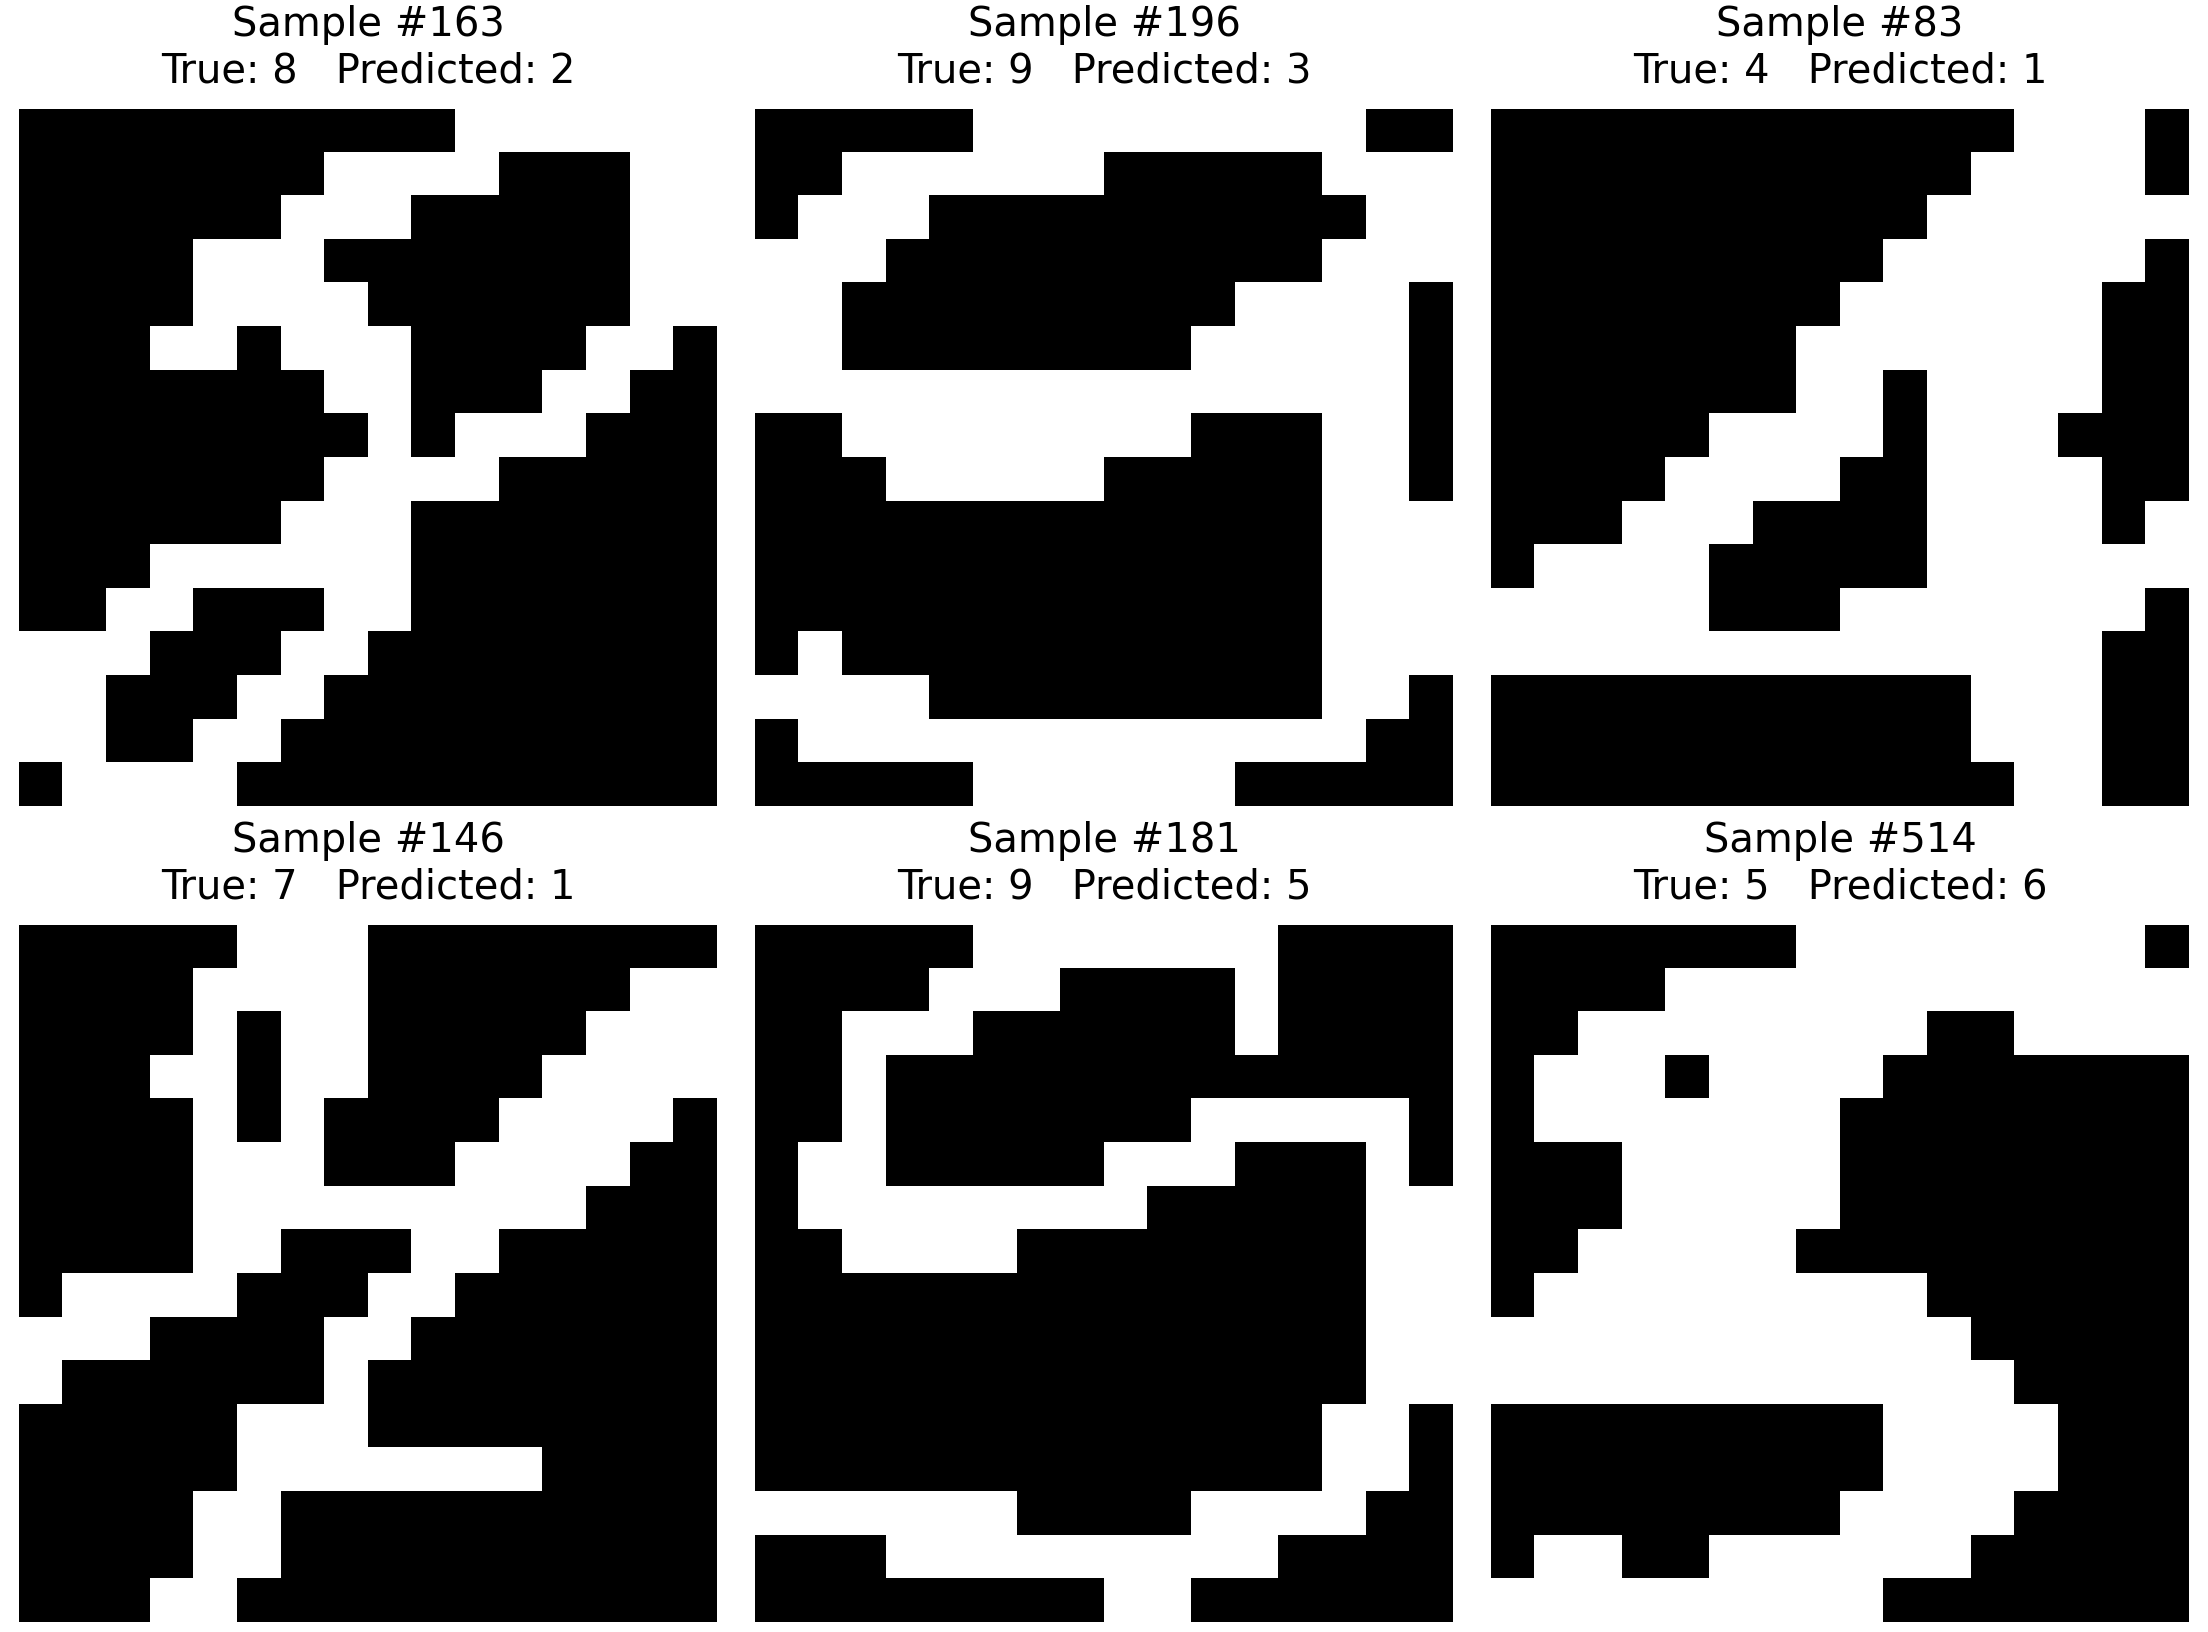
\includegraphics[width=0.92\textwidth]{local_errors_k1.png}
  \caption{自写 kNN 在补充复核运行中的错分类样本：True 为真实标签，Predicted 为预测标签}
  \label{fig:local-errors}
\end{figure}

\begin{table}[H]
  \centering
  \caption{展示样本所属的主要混淆类型及出现次数}
  \label{tab:error-pairs}
  \begin{tabular}{cccc}
    \toprule
    原始行号 & 真实类别 & 预测类别 & 该类型错误总数 \\
    \midrule
    163 & 8 & 2 & 15 \\
    196 & 9 & 3 & 14 \\
    83 & 4 & 1 & 11 \\
    146 & 7 & 1 & 9 \\
    181 & 9 & 5 & 8 \\
    514 & 5 & 6 & 6 \\
    \bottomrule
  \end{tabular}
\end{table}

这些图像可见环状结构、横向笔画及斜向主笔画的写法差异。在 $16\times16$ 二值表示中，环的闭合程度和少量像素变化可能改变不同数字之间的距离。逐像素欧氏距离也未显式建模笔画结构或平移不变性，因此形态近似可能影响近邻选择。这是基于图像的可能解释，尚不能单独证明各样本的具体误分类原因；进一步分析需展示其选中的近邻或做特征对照实验。

生成脚本为 \path{report/generate_error_figures.py}，在项目根目录用 Python 运行即可生成三个混淆矩阵和一张 $k=1$ 错样本图，同时保存每个 $k$ 的逐样本预测 CSV、混淆矩阵 CSV 及 \path{report/error_figure_summary.json}。文件名中的 k1、k3、k5 标明对应参数。程序逐组检查矩阵总和、各行类别数量及正确数，并确认所有展示样本确实预测错误，避免图像与统计结果来自不同批次。

\section{踩坑记录与解决方法}

\subsection{数据准备阶段}

\textbf{坑 1：分不清三个数据文件的关系。} 文件夹中同时出现完整数据和 train/test 划分文件，容易误用固定划分进行实验。解决方法是用 NumPy 逐行比对确认 train/test 合并后等于全集，并根据 LOO 要求只使用 \texttt{semeion.data}。

\textbf{坑 2：注释写“随机画 6 张”，实际永远画前 6 张。} 原示例使用 \texttt{range(6)}，文件开头的样本标签均为 0，因此重复运行显示的类别不变。解决方法是随机抽取下标。进一步核查确认数字 0 总计 161 个、文件开头连续为 0 的样本为 20 个，不能把类别总数当作连续排列长度。

\subsection{代码实现阶段}

\textbf{坑 3：LOO 性能问题。} 1593 轮 LOO 每轮都要计算 1592 个训练样本到测试样本的 256 维距离，纯 Python 双重循环会较慢。解决方法是使用 NumPy 广播向量化距离计算，使每轮的距离计算由底层数组运算完成。

\subsection{结果验证阶段}

\textbf{坑 4：输出与文档“预期结果”不符。} 自写程序得到约 91\% 的准确率，而导论文档预期约 98.5\%。解决方法是从代码、数据、工具和实验协议四个层面核查。已有结果支持约 91\% 的实测水平，但无法确定预期值的来源；不据此调整数据或评估协议。

\subsection{Weka 对比阶段}

\textbf{坑 5：用 Weka 打开 \texttt{semeion.names} 报错。} \texttt{.names} 是说明文档，不是数据文件；Weka 会按 C4.5 格式解析，失败是正常的。解决方法是将 \texttt{semeion.data} 转换为 ARFF。

\textbf{坑 6：混淆距离加权与训练池窗口参数。} 距离加权会改变投票规则，应核对 \texttt{distanceWeighting = No distance weighting}；而 \texttt{-W 0} 只表示训练池大小不受窗口限制。外部 LOO 应通过 Explorer 的 Cross-validation 设置 1593 折实现，不通过 IBk 内部自动选择 $k$ 的选项实现。

\textbf{坑 7：Weka 与原始自写结果仍有约 0.25 个百分点差异。} 差异低于导论阈值，可能与距离并列及投票平局有关。补充复核证实排序规则能影响精度，但尚未将 Weka 的逐样本误差归因到具体规则。经验是同时保存实验配置和逐样本预测，避免只凭总体精度判断差异来源。

\section{结论}

本实验完成了基于 kNN 的 Semeion 手写数字识别任务。通过自写 Python 程序，在完整数据集上使用留一法得到 $k=1$、$k=3$、$k=5$ 的准确率分别为 91.90\%、90.46\%、90.46\%。Weka IBk 在相同协议下得到 91.6510\%、90.2072\%、90.7094\%，与自写实现差异均小于 0.5\%。

实验结果表明，在该数据集及当前评估设置下 $k=1$ 的表现最好，扩大邻域并未提升分类准确率。默认参数、数据格式和评估协议均会影响结果比较，因此需统一实验设置，并结合运行记录核查结果。

修订阶段的环境复核得到略有差异的数值，并通过排序对照确认等距离邻居处理具有影响。该补充实验提高了对复现条件的认识，但不能替代对原始环境的完整记录。$k=1$ 是本次比较中的最优值；若进一步据此选择模型，应使用独立测试集或嵌套验证评价所选模型，避免将同一组用于选参的结果直接作为最终泛化估计。

\section*{参考资料}
\addcontentsline{toc}{section}{参考资料}

\begin{enumerate}[label={[\arabic*]}]
  \item UCI Machine Learning Repository. Semeion Handwritten Digit Data Set. \url{http://archive.ics.uci.edu/ml/datasets/Semeion+Handwritten+Digit}
  \item 课程材料：《机器学习》课程实验一导论，基于 kNN 的手写数字识别实验。
  \item 课程材料：KNN 算法基础概念课件。
  \item Weka Explorer 输出结果：IBk 分类器，$k=1,3,5$，1593-fold cross-validation。
  \item Weka. IBk API Documentation. \url{https://weka.sourceforge.io/doc.stable/weka/classifiers/lazy/IBk.html}
  \item NumPy. numpy.argsort Documentation. \url{https://numpy.org/doc/1.26/reference/generated/numpy.argsort.html}
\end{enumerate}

\appendix
\section{附录：本地运行输出}

\begin{lstlisting}[basicstyle=\ttfamily\small,backgroundcolor=\color{codebg},frame=single,breaklines=true]
(ml) PS E:\browser\machine_learning\Lab1> python exp_1.py
样本数: 1593 | 特征数(像素): 256 | 前10个标签: [0 0 0 0 0 0 0 0 0 0]
k=1  LOO 准确率 = 0.9190
k=3  LOO 准确率 = 0.9046
k=5  LOO 准确率 = 0.9046
\end{lstlisting}

\end{document}
